%==========================================================
\section{Casos de uso}\label{sec:casosdeuso}

%----------------------------------------------------------
% Não é o diagrama de contexto do Contextual Design (nota do enunciado).
\subsection{Diagrama de contexto (nível 0)}\label{sec:contexto}

\begin{figure}[H]
\centering
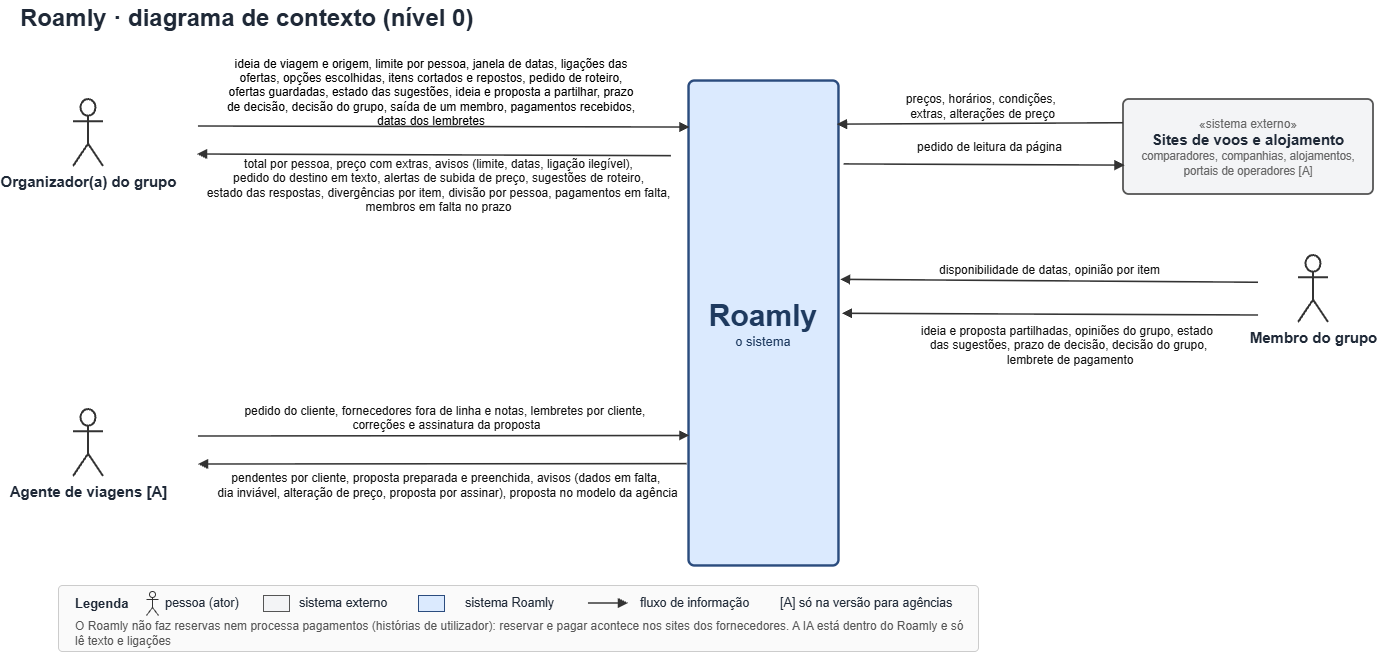
\includegraphics[width=\textwidth]{diagramas/diagrama_contexto_nivel0/Roamly-diagrama-contexto-N0.drawio.png}
\caption{Diagrama de contexto (nível 0) do \projeto.}
\label{fig:contexto}
\end{figure}


%----------------------------------------------------------
\subsection{Diagrama de casos de uso (nível 1)}\label{sec:diagrama-uc}

O diagrama da Figura~\ref{fig:diagrama-uc} mostra os casos de uso da Release~1, derivados das histórias da
Secção~\ref{sec:storymap}. O organizador do grupo é o ator principal e está ligado aos objetivos que inicia. Os membros do
grupo e os sites dos fornecedores são atores secundários: o Roamly precisa deles para cumprir o objetivo. Os sites dos
fornecedores são um sistema externo, por isso estão marcados com \guillemotleft sistema\guillemotright. Cada caso de uso indica
o seu nível de Cockburn. As relações \guillemotleft include\guillemotright{} e \guillemotleft extend\guillemotright{} mostram o
comportamento partilhado (calcular o total por pessoa) e o opcional (cortar um item, alertar a subida de preço), com os pontos
de extensão indicados nos casos base.

\begin{figure}[H]
\centering
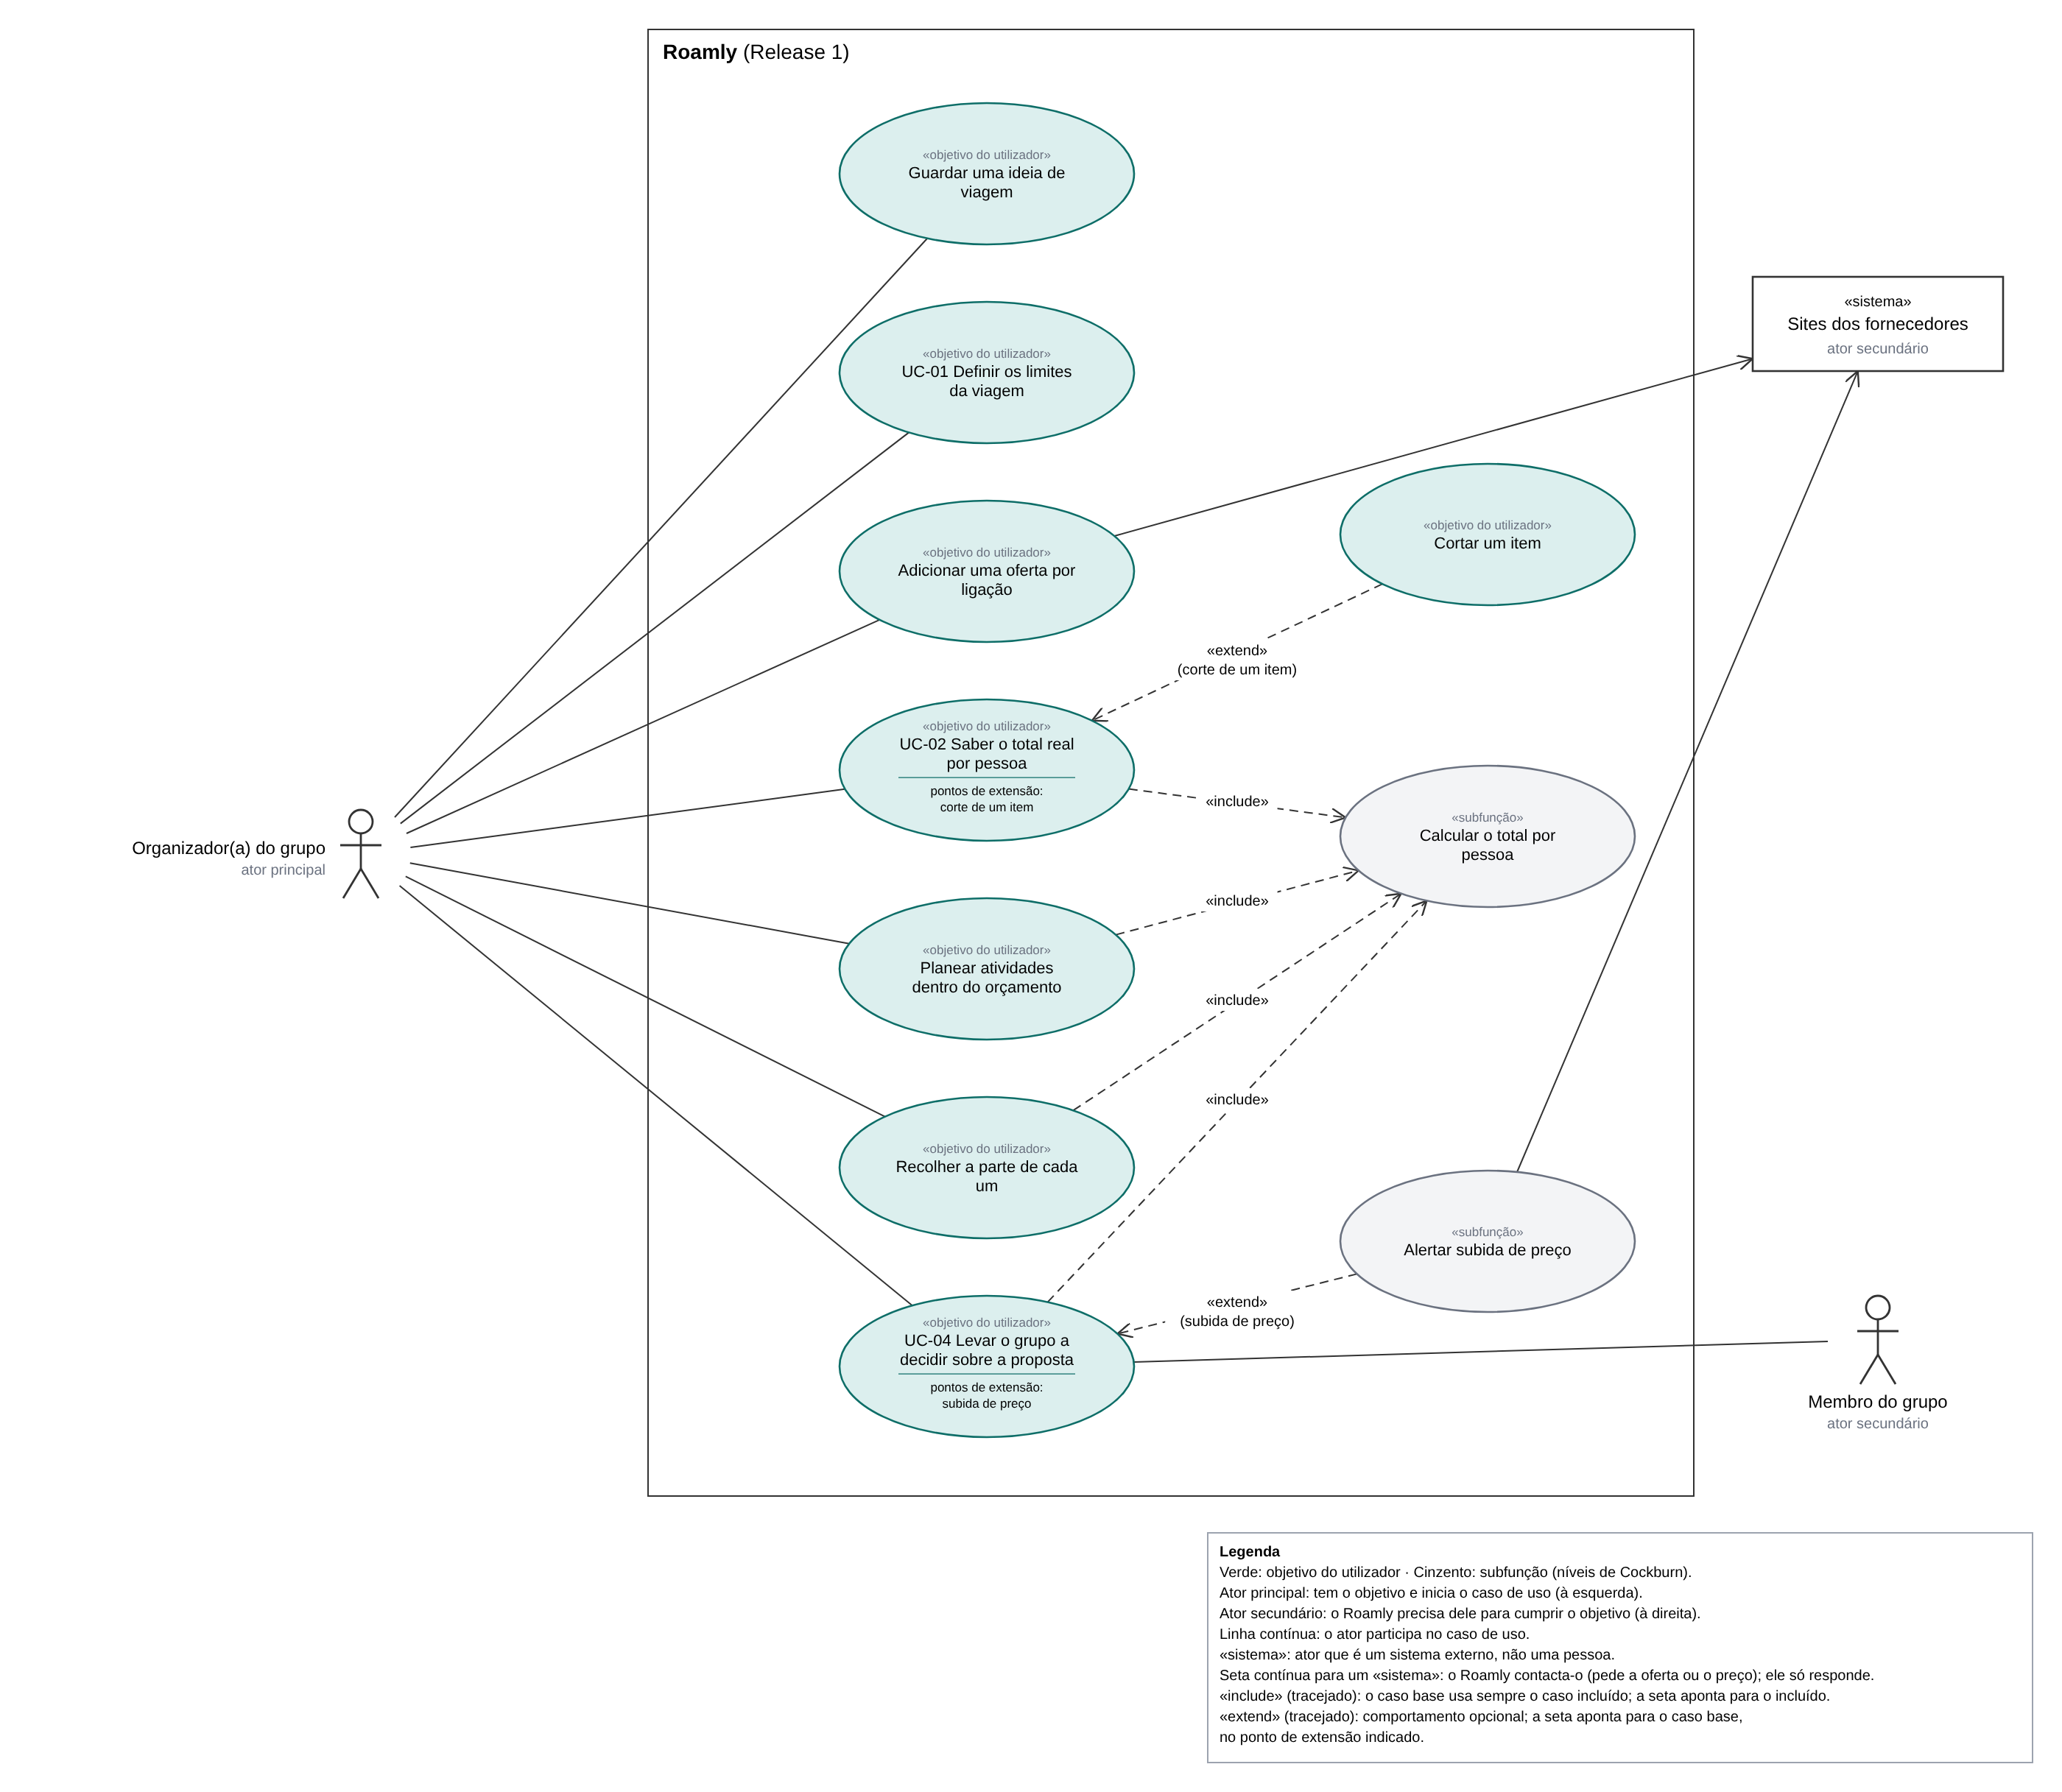
\includegraphics[width=\textwidth]{diagramas/diagrama-nivel1/use-case-diagram.png}
\caption{Diagrama de casos de uso do \projeto{} (Release 1).}
\label{fig:diagrama-uc}
\end{figure}

%----------------------------------------------------------
\subsection{Casos de uso detalhados}\label{sec:uc-detalhados}

Os três casos de uso detalhados cobrem as histórias de maior prioridade da Release~1: definir os limites da viagem (UC-01),
saber o total real por pessoa (UC-02) e levar o grupo a decidir sobre a proposta (UC-04). Seguem o modelo de Cockburn e
cada um indica as histórias, a sequência consolidada, as funções do UED e os \textit{breakdowns} em que se baseia.

% Fonte: ../casos_de_uso/corrigidos/ (os originais, gerados por IA, estão em ../casos_de_uso/)
\begingroup
\setlength{\parindent}{0pt}
\setlength{\parskip}{4pt}
\clearpage
\documentclass[11pt,a4paper]{article}
\usepackage[utf8]{inputenc}
\usepackage[T1]{fontenc}
\usepackage[portuguese]{babel}
\usepackage{lmodern}
\usepackage[margin=2.3cm]{geometry}
\usepackage{tabularx,booktabs,array,enumitem}
\usepackage[table]{xcolor}
\usepackage{textcomp}
\usepackage{hyperref}

\definecolor{roamly}{HTML}{0E6E68}
\definecolor{pendente}{HTML}{6B7280}
\hypersetup{colorlinks=true,linkcolor=roamly,urlcolor=roamly}
\newcolumntype{L}{>{\raggedright\arraybackslash}X}
\renewcommand{\arraystretch}{1.3}
\setlist{nosep,leftmargin=*}
\setlength{\parindent}{0pt}
\setlength{\parskip}{4pt}

% reference to an interview record or a breakdown (as in the report)
\newcommand{\reg}[1]{{\footnotesize\textcolor{pendente}{(#1)}}}
% use case
\newenvironment{usecase}[2]{%
  \par\medskip\noindent{\large\bfseries\color{roamly}#1: #2}\par\smallskip\small\noindent\ignorespaces}{\par\medskip}
\newcommand{\ucField}[2]{\textbf{#1} & #2 \\}

\begin{document}

\begin{usecase}{UC-01}{Definir os limites da viagem}
\textbf{Descrição breve.} Antes de procurar opções, o organizador do grupo indica quanto cada pessoa pode gastar e em que datas o grupo pode viajar. O sistema guarda estes limites na viagem e compara com eles tudo o que o organizador juntar depois. Assim, a viagem parte do orçamento e das datas do grupo, e não de um destino.\par\smallskip
\begin{tabularx}{\textwidth}{@{}>{\raggedright\arraybackslash}p{3.4cm}L@{}}
\toprule
\ucField{Ator principal}{Organizador(a) do grupo}
\ucField{Atores secundários}{Nenhum}
\ucField{Nível}{Objetivo do utilizador}
\ucField{Âmbito}{Roamly (versão base, viajante)}
\ucField{Área de foco}{1. Explorar ideias}
\ucField{Gatilho}{O grupo responde à ideia de viagem com as suas condições de preço e de datas («depende do preço; era mais fácil perto do fim de semana») \reg{UE02}.}
\ucField{Pré-condições}{Existe uma ideia de viagem guardada no Roamly («Guardar uma ideia de viagem», US-01). A viagem ainda não precisa de ter destino.}
\ucField{Garantia mínima}{O limite por pessoa e as datas já indicados ficam guardados. Nenhuma opção é comparada com um limite que o organizador não indicou.}
\ucField{Garantia de sucesso}{A viagem tem um limite por pessoa e uma janela de datas. Cada opção que o organizador juntar é comparada com eles, e o total por pessoa (UC-02) tem um limite com que ser comparado.}
\bottomrule
\end{tabularx}

\medskip
\textbf{Partes interessadas e interesses}
\begin{itemize}
  \item \textbf{Organizador(a) do grupo:} planear uma viagem barata que todo o grupo aceite, até 300\,€ por pessoa; partir do orçamento e das datas, e não do destino \reg{UE03, U0-05}; não ter de refazer tudo à mão quando uma condição muda \reg{UE09}.
  \item \textbf{Membros do grupo:} não ficarem presos a uma viagem acima do que podem pagar ou em datas em que não podem ir \reg{UE02, U0-03}.
  \item \textbf{Família (guardião financeiro):} «não gastes o que não tens» \reg{U0-12}.
\end{itemize}

\textbf{Cenário principal de sucesso}
\begin{enumerate}
  \item O organizador indica quanto cada pessoa pode gastar (p.\,ex., até 300\,€ por pessoa).
  \item O sistema guarda o limite por pessoa na viagem.
  \item O organizador indica as datas em que o grupo pode viajar.
  \item O sistema guarda a janela de datas na viagem.
\end{enumerate}

\textbf{Extensões}
\begin{itemize}[leftmargin=2.2em]
  \item[1a.] \textit{Ainda não se sabe quanto o grupo pode gastar} («depende do preço», \reg{UE02}): o organizador avança sem limite. Sempre que junta uma opção, o sistema lembra-o de que não há limite com que a comparar (US-02). Continua no passo 3.
  \item[3a.] \textit{O grupo pode ir em qualquer altura de um período} («mês inteiro», \reg{UE03, U0-05}): o organizador indica o período inteiro como janela de datas, sem destino fixo. Continua no passo 4.
  \item[*a.] \textit{As datas possíveis mudam depois de já haver opções na viagem} (o Amigo~B só pode a partir de uma sexta-feira concreta, \reg{UE09, U0-03}): o organizador indica a nova janela de datas (passo 3). O sistema volta a comparar as opções já juntas com as novas datas e avisa das que ficaram fora (US-28).
\end{itemize}

\textbf{Rastreabilidade}
\begin{itemize}
  \item \textbf{Histórias:} US-02 «Definir o limite por pessoa» (passos 1 e 2; 1a); US-28 «Definir a janela de datas» (passos 3 e 4; 3a, *a).
  \item \textbf{Sequência consolidada:} atividade 2 «Perceber o que quem viaja quer», passo «Saber o orçamento, as datas e o que não se abdica» (intenção: perceber o que quem viaja quer e até onde é flexível); atividade 3, pesquisa com datas «mês inteiro» \reg{UE03} (3a); atividade 7, «Refazer quando uma condição muda» \reg{UE09} (*a).
  \item \textbf{UED, área 1:} «Indicar o orçamento por pessoa, as datas possíveis e o que não se dispensa» (passos 1 a 4); «Pesquisar só por orçamento e datas, sem destino fixo» (3a). Ligação da área 5 para a área 1, «para refazer a pesquisa com novas datas» (*a).
  \item \textbf{Afinidade:} «Tenho orgulho em gastar menos».
  \item \textbf{\textit{Breakdowns}:} SM.11, AM.26 (ver nota 2).
  \item \textbf{Persona:} Inês.
\end{itemize}
\end{usecase}

\medskip
{\footnotesize\textbf{Notas para revisão.}
(1) O ator principal usa o nome das histórias e do diagrama de casos de uso. No modelo de fluxo consolidado, este objetivo junta o planeamento da viagem e a coordenação do grupo; nesta entrega, ambos são do organizador.
(2) Os \textit{breakdowns} da área 1 são SM.11 e AM.26: o roteiro do cliente não diz o orçamento, as datas flexíveis nem «o que não abdicam» \reg{A0-06}. São do agente e não entram neste caso de uso (versão base). A variante do agente é a US-03 [A] (Release~3).
(3) A função do UED da área 1 inclui também «o que não se dispensa». Fica fora deste caso de uso: só o agente mostra esse dado \reg{A0-06}, o caso do viajante não mostra o grupo a fixá-lo à partida, e nenhuma história da Release~1 o pede.
(4) O que acontece quando o organizador junta uma opção pertence a «Adicionar uma oferta por ligação»: o aviso de opção fora da janela de datas (US-28) é dessa altura. O aviso de total acima do limite está no UC-02 (4b).
(5) Não há atores secundários. Os membros do grupo dão as suas condições na conversa do grupo, fora do Roamly (é o gatilho, \reg{UE02}), e a família não usa o Roamly. Por isso estão nas partes interessadas, e não nos atores.\par}

\end{document}

\clearpage
\documentclass[11pt,a4paper]{article}
\usepackage[utf8]{inputenc}
\usepackage[T1]{fontenc}
\usepackage[portuguese]{babel}
\usepackage{lmodern}
\usepackage[margin=2.3cm]{geometry}
\usepackage{tabularx,booktabs,array,enumitem}
\usepackage[table]{xcolor}
\usepackage{textcomp}
\usepackage{hyperref}

\definecolor{roamly}{HTML}{0E6E68}
\definecolor{pendente}{HTML}{6B7280}
\hypersetup{colorlinks=true,linkcolor=roamly,urlcolor=roamly}
\newcolumntype{L}{>{\raggedright\arraybackslash}X}
\renewcommand{\arraystretch}{1.3}
\setlist{nosep,leftmargin=*}
\setlength{\parindent}{0pt}
\setlength{\parskip}{4pt}

% reference to an interview record or a breakdown (as in the report)
\newcommand{\reg}[1]{{\footnotesize\textcolor{pendente}{(#1)}}}
% use case
\newenvironment{usecase}[2]{%
  \par\medskip\noindent{\large\bfseries\color{roamly}#1: #2}\par\smallskip\small\noindent\ignorespaces}{\par\medskip}
\newcommand{\ucField}[2]{\textbf{#1} & #2 \\}

\begin{document}

\begin{usecase}{UC-02}{Saber o total real por pessoa}
\textbf{Descrição breve.} Depois de escolher as opções da viagem, o organizador do grupo quer saber quanto custa de facto a cada pessoa e se a viagem cabe no limite. O sistema soma num só sítio o preço das opções escolhidas, já com os extras, compara o total por pessoa com o limite da viagem e mantém-no atualizado quando um preço muda ou um item é cortado. Assim, o organizador deixa de copiar preços à mão para uma folha de cálculo e não tem surpresas na página de pagamento.\par\smallskip
\begin{tabularx}{\textwidth}{@{}>{\raggedright\arraybackslash}p{3.4cm}L@{}}
\toprule
\ucField{Ator principal}{Organizador(a) do grupo}
\ucField{Atores secundários}{Sites dos fornecedores (sistema externo): o sistema volta a ler as ofertas escolhidas para saber se o preço mudou (*a, *c)}
\ucField{Nível}{Objetivo do utilizador}
\ucField{Âmbito}{Roamly (versão base, viajante)}
\ucField{Área de foco}{3. Orçamento da viagem}
\ucField{Gatilho}{O organizador escolheu voo e alojamento e quer saber se a viagem cabe no limite por pessoa \reg{UE06}.}
\ucField{Pré-condições}{A viagem tem pelo menos um voo ou um alojamento guardado a partir da ligação da oferta, com o preço por pessoa lido da página ou preenchido à mão («Adicionar uma oferta por ligação», US-04, US-05). O limite por pessoa (UC-01) pode ainda não estar definido (extensão 4a).}
\ucField{Garantia mínima}{Nenhum custo conhecido fica fora do total. O que falta ou está por confirmar fica assinalado no total, em vez de ser omitido. Um item cortado não se perde.}
\ucField{Garantia de sucesso}{O organizador vê num só sítio o total por pessoa, com os extras, e se cabe no limite. O total fica na proposta, atualizado, pronto para o grupo decidir (UC-04).}
\bottomrule
\end{tabularx}

\medskip
\textbf{Partes interessadas e interesses}
\begin{itemize}
  \item \textbf{Organizador(a) do grupo:} saber se a viagem cabe nos 300\,€ por pessoa sem refazer as contas à mão \reg{UE06, UE09, UE12}; ter num só sítio o custo que hoje está espalhado pelo comparador, pelo transporte e pela folha de cálculo \reg{U0-07}; não ter surpresas na página de pagamento («isto ninguém diz», \reg{UE07, U0-08}).
  \item \textbf{Membros do grupo:} decidir com base no preço real («depende do preço», \reg{UE02}); perceber o que foi cortado e porquê \reg{UE12, U0-17}.
  \item \textbf{Família (guardião financeiro):} «não gastes o que não tens» \reg{U0-12}.
\end{itemize}

\textbf{Cenário principal de sucesso}
\begin{enumerate}
  \item O organizador escolhe as opções que entram na viagem: voo, alojamento e atividades.
  \item O sistema calcula o total por pessoa das opções escolhidas, já com os extras de cada oferta, como a bagagem de porão (inclui «Calcular o total por pessoa»).
  \item O sistema mostra ao organizador, num só sítio, o total por pessoa e de que é feito: o preço de cada opção e os seus extras.
  \item O sistema compara o total por pessoa com o limite da viagem (UC-01) e mostra ao organizador que a viagem cabe no limite.
  \item O sistema guarda o total por pessoa na proposta, pronto para ser partilhado com o grupo (UC-04).
\end{enumerate}

\textbf{Extensões}
\begin{itemize}[leftmargin=2.2em]
  \item[2a.] \textit{O site não revela o preço dos extras de uma oferta} (\reg{FM.1, SM.16, CM.31}): o sistema conta a oferta no total e indica que os extras estão por confirmar, em vez de os omitir (US-06). Continua no passo 3.
  \item[2b.] \textit{(Release 2, US-29) Um voo obriga a apanhar transporte até ao aeroporto} (comboio e metro, cerca de 13\,€ por sentido, \reg{UE04; AM.24, SM.14}): o custo desse transporte entra no total por pessoa. Se o custo não é conhecido, o total indica que falta esse custo. Continua no passo 3.
  \item[4a.] \textit{A viagem ainda não tem limite por pessoa} («depende do preço», \reg{UE02}; UC-01, 1a): o sistema mostra o total por pessoa sem o comparar e lembra o organizador de que não há limite com que o comparar (US-02). Continua no passo 5.
  \item[4b.] \textit{O total por pessoa passa o limite} (303\,€ para um limite de 300\,€, \reg{UE06}): o sistema avisa o organizador de que passou o limite (US-09). O organizador corta um item (*b) ou troca uma opção (área 2, «Comparar opções»), e o sistema volta ao passo 2.
  \item[*a.] \textit{O preço de uma opção escolhida muda} (o voo subiu 19\,€, \reg{UE08}), ou as datas mudam e as opções são refeitas (322\,€ depois de o Amigo~B mudar as datas, \reg{UE09}): o sistema deteta a mudança quando volta a ler a oferta no site do fornecedor, ou quando o organizador refaz as opções. Atualiza sozinho o total por pessoa (US-09) e volta a compará-lo com o limite (passo 4).
  \item[*b.] \textit{O organizador corta um item}; ponto de extensão \textit{corte de um item} («Cortar um item», US-10): o organizador corta a visita à mina de sal (28\,€, «isto é para turistas», \reg{UE12}). O sistema tira o item do total, que passa logo de 322\,€ para 294\,€, e o item continua visível como cortado, para o grupo ver o que saiu e porquê \reg{U0-17}. Se o organizador repuser o item, o total volta ao valor anterior. Continua no passo 3.
  \item[*c.] \textit{O sistema já não consegue ler uma oferta escolhida no site do fornecedor}: o total por pessoa mantém o último preço conhecido dessa oferta e indica que pode estar desatualizado (US-08). Continua no passo 3.
\end{itemize}

\textbf{Rastreabilidade}
\begin{itemize}
  \item \textbf{Histórias:} US-09 «Ver o total por pessoa» (passos 1 a 5; 4b, *a); US-06 «Ver o preço final com extras» (passos 2 e 3; 2a); US-10 «Cortar um item e ver o efeito» (*b); US-02 «Definir o limite por pessoa» (4a); US-08 «Alertar quando o preço sobe», critério 2 (*c); US-29 «Contar o transporte até ao aeroporto no total», Release~2 (2b).
  \item \textbf{Sequência consolidada:} atividade 5 «Juntar tudo numa proposta» (intenção: ter depressa uma proposta cujo total por pessoa caiba no orçamento), passos «Copiar os dados de outros sistemas para a proposta» \reg{UE06} e «Ver o custo real» \reg{UE07}; atividade 4, «Verificar a logística» \reg{UE04} (2b); atividade 7, «Cortar o que não cabe» \reg{UE12} (*b) e «Refazer quando uma condição muda» \reg{UE09} (*a).
  \item \textbf{UED, área 3:} «Somar o total por pessoa» (passos 2 e 3); «Avisar quando o total passa o orçamento por pessoa» (4, 4b); «Cortar um item e ver o efeito no total» (*b); «Atualizar o total quando um preço muda» (*a); «Incluir o transporte até ao aeroporto» (2b). Área 2: «Mostrar o preço final, já com extras como a bagagem de porão» (2, 2a); ligação da área 2 para a área 3 (4b).
  \item \textbf{Afinidade:} «Faço e refaço as contas eu mesmo/a»; «Copio à mão de um sistema para outro»; «Os extras só aparecem quando vou pagar»; «O custo de chegar ao aeroporto fica fora das minhas contas».
  \item \textbf{\textit{Breakdowns} (área 3):} SM.14 (passos 2 e 3; 2b); AM.24 (2b); FM.7, SM.15, AM.23, PM.28 (ver nota 2). Da área 2, por tocarem neste objetivo: FM.1, SM.16, CM.31 (2a).
  \item \textbf{Diagrama de casos de uso (L1):} inclui «Calcular o total por pessoa»; é estendido por «Cortar um item» no ponto de extensão \textit{corte de um item}; ator secundário: sites dos fornecedores.
  \item \textbf{Persona:} Inês.
\end{itemize}
\end{usecase}

\medskip
{\footnotesize\textbf{Notas.}
(1) Os sites dos fornecedores são ator secundário porque, nas extensões *a e *c, o sistema volta a ler as ofertas escolhidas para saber se o preço mudou. Os membros do grupo não são atores: não usam o Roamly neste caso de uso.
(2) FM.7, SM.15, AM.23 e PM.28 descrevem o agente a copiar à mão os dados do portal para a proposta \reg{AE05, A0-07}. Na versão base, o mesmo problema existe do lado do organizador, que copia à mão os preços de cada site para a folha de cálculo \reg{UE06}, e fica resolvido pelo cenário principal: o total é calculado a partir das ofertas guardadas, sem cópia. A variante do agente é a US-30 [A] (Release~3).
(3) A extensão 2b depende da US-29, que é da Release~2 e tem um \textit{spike} sobre a fonte de horários e preços de transportes; fica no caso de uso para mostrar desde já onde entra esse custo.
(4) O ator principal usa o nome das histórias e do diagrama de casos de uso. No modelo de fluxo consolidado, este objetivo é do papel \textit{Planeador da viagem}.
(5) O corte de um item é a extensão *b, e não 4c, porque pode acontecer em qualquer passo, e não só quando o total passa o limite.\par}

\end{document}

\clearpage
\documentclass[11pt,a4paper]{article}
\usepackage[utf8]{inputenc}
\usepackage[T1]{fontenc}
\usepackage[portuguese]{babel}
\usepackage{lmodern}
\usepackage[margin=2.3cm]{geometry}
\usepackage{tabularx,booktabs,array,enumitem}
\usepackage[table]{xcolor}
\usepackage{textcomp}
\usepackage{hyperref}

\definecolor{roamly}{HTML}{0E6E68}
\definecolor{pendente}{HTML}{6B7280}
\hypersetup{colorlinks=true,linkcolor=roamly,urlcolor=roamly}
\newcolumntype{L}{>{\raggedright\arraybackslash}X}
\renewcommand{\arraystretch}{1.3}
\setlist{nosep,leftmargin=*}
\setlength{\parindent}{0pt}
\setlength{\parskip}{4pt}

% reference to an interview record or a breakdown (as in the report)
\newcommand{\reg}[1]{{\footnotesize\textcolor{pendente}{(#1)}}}
% use case
\newenvironment{usecase}[2]{%
  \par\medskip\noindent{\large\bfseries\color{roamly}#1: #2}\par\smallskip\small\noindent\ignorespaces}{\par\medskip}
\newcommand{\ucField}[2]{\textbf{#1} & #2 \\}

\begin{document}

\begin{usecase}{UC-04}{Levar o grupo a decidir sobre a proposta}
\textbf{Descrição breve.} O organizador do grupo partilha a proposta de viagem com os amigos que vão. Cada membro indica em que datas pode ir e se aceita cada item, e o organizador regista o que o grupo combinou. O sistema mostra a todos a mesma proposta e o mesmo total por pessoa, mostra ao organizador quem já respondeu e onde o grupo diverge, e guarda a decisão na proposta. A seguir, o organizador pode sair do Roamly para reservar no site de cada fornecedor.\par\smallskip
\begin{tabularx}{\textwidth}{@{}>{\raggedright\arraybackslash}p{3.4cm}L@{}}
\toprule
\ucField{Ator principal}{Organizador(a) do grupo}
\ucField{Atores secundários}{Membros do grupo (indicam as suas datas e a sua opinião sobre cada item)}
\ucField{Nível}{Resumo: a decisão demora dias e faz-se em várias sessões, de pessoas diferentes \reg{UE08}}
\ucField{Âmbito}{Roamly (versão base, viajante)}
\ucField{Área de foco}{5. Decidir com o grupo ou o cliente}
\ucField{Gatilho}{A proposta cabe no limite por pessoa (UC-02) e o organizador quer a decisão do grupo antes de o preço mudar.}
\ucField{Pré-condições}{A viagem tem uma proposta com o total por pessoa (UC-02) e os seus limites (UC-01). O organizador sabe quem vai.}
\ucField{Garantia mínima}{As datas e as opiniões já dadas ficam guardadas. Todos os membros veem a mesma versão, atual, da proposta.}
\ucField{Garantia de sucesso}{O que o grupo combinou fica registado na proposta, junto dos itens a que se refere, e todos os membros o veem. O organizador sabe a resposta de cada um e pode sair do Roamly para reservar no site de cada fornecedor.}
\bottomrule
\end{tabularx}

\medskip
\textbf{Partes interessadas e interesses}
\begin{itemize}
  \item \textbf{Organizador(a) do grupo:} ter uma decisão antes de o preço subir \reg{UE08}; saber a quem insistir sem perguntar um a um \reg{UE08}; não ser o único a lembrar-se, depois de cada conversa, do que ficou combinado \reg{UE18, U0-19}.
  \item \textbf{Membros do grupo:} responder sem abrir folhas de cálculo («manda print») \reg{UE17}; dizer o que não aceitam («dormitório não») antes de se reservar alguma coisa \reg{UE05}; dizer quando podem ir \reg{UE02, UE09}.
\end{itemize}

\noindent\begin{minipage}{\textwidth}
\setlength{\parskip}{4pt}
\textbf{Cenário principal de sucesso}

Cada passo está na coluna de quem o faz. Os passos 3 e 4 são feitos por cada membro, no seu tempo.

\begin{tabularx}{\textwidth}{@{}>{\raggedleft\arraybackslash}p{0.5cm}LLL@{}}
\toprule
 & \textbf{Organizador(a) do grupo} & \textbf{Membros do grupo} & \textbf{Sistema} \\
\midrule
1. & Partilha a proposta com o grupo. & & \\
2. & & & Mostra a proposta a cada membro: itens, preços, total por pessoa e o que foi cortado e porquê. \\
3. & & Cada membro indica se pode ir nas datas propostas ou em que outras datas pode. & \\
4. & & Cada membro indica se aceita cada item. & \\
5. & & & Mostra ao organizador quem já respondeu, quem ainda falta e os itens em que os membros divergem. \\
6. & Regista na proposta o que o grupo combinou. & & \\
7. & & & Guarda a decisão na proposta e mostra-a a todos os membros, junto dos itens a que se refere. \\
\bottomrule
\end{tabularx}
\end{minipage}

\textbf{Extensões}
\begin{itemize}[leftmargin=2.2em]
  \item[2a.] \textit{Um membro não abre a proposta partilhada} («manda print», \reg{UE17; FM.9, SM.21, AM.25}): o organizador envia um resumo com o total por pessoa que se lê na própria conversa do grupo (US-14). Continua no passo 5, onde esse membro continua a aparecer em falta.
  \item[3a.] \textit{Um membro só pode ir noutras datas} (o Amigo~B só pode a partir de uma sexta-feira concreta, \reg{UE09, U0-03}): o sistema regista essas datas como alternativa às propostas (US-15) e mostra-as ao organizador junto da resposta desse membro (US-31). Se o organizador refizer a pesquisa, a janela de datas muda no UC-01 (*a) e a proposta atualizada volta a ser partilhada (passo 1).
  \item[4a.] \textit{Um membro não aceita um item} («dormitório não», \reg{UE05}): a resposta do membro fica visível ao grupo junto desse item, e o sistema mostra ao organizador em que itens há divergência (US-16). O organizador troca a opção (área 2, «Comparar opções») e o grupo vê a proposta atualizada (*a), ou mantém-no e continua no passo 6.
  \item[5a.] \textit{Os membros demoram a responder} (dois dias sem resposta, \reg{UE08; FM.8}): o organizador vê quem ainda falta (US-31) e insiste só com esses. Continua no passo 3 para esses membros.
  \item[5b.] \textit{(Release 2, US-17) O prazo fixado pelo organizador passa e falta alguém responder}: o sistema avisa o organizador de quem falta. Continua em 5a ou no passo 6.
  \item[6a.] \textit{O grupo decide ao vivo, à volta de um só telemóvel} (no café, \reg{UE18; SM.22, PM.29}): o organizador regista o combinado na proposta naquele momento (US-18). Continua no passo 7.
  \item[6b.] \textit{Há membros que ainda não responderam quando o organizador regista a decisão}: a decisão fica registada e esses membros também a veem (US-18). Continua no passo 7.
  \item[*a.] \textit{O organizador altera um item depois de partilhar a proposta}: quem abre a proposta vê a versão atualizada (US-14), com o novo total por pessoa.
  \item[*b.] \textit{O preço de uma opção sobe enquanto o grupo decide} (o voo subiu 19\,€: «malta, subiu», \reg{UE08; FM.2, SM.17}); ponto de extensão \textit{subida de preço}: o sistema avisa o organizador e os membros e mostra de quanto subiu, sem mensagens de urgência (US-08, «Alertar subida de preço»). O total por pessoa é atualizado e o grupo vê-o na proposta (*a).
\end{itemize}

\textbf{Rastreabilidade}
\begin{itemize}
  \item \textbf{Histórias:} US-14 (passos 1 e 2; 2a, *a); US-15 (passo 3; 3a); US-16 (passo 4; 4a); US-31 (passo 5; 3a, 5a); US-18 (passos 6 e 7; 6a, 6b); US-08 (*b); US-17, Release~2 (5b).
  \item \textbf{Sequência consolidada:} atividade 6 «Levar a proposta a quem decide» (intenção: conseguir uma decisão de quem viaja antes que o preço mude) e o seu \textit{breakdown} «o grupo responde devagar e o preço sobe» \reg{U0-09}; atividade 9, «Pôr o grupo a par das contas» \reg{UE17} e «Escolher o resto em conjunto e registá-lo» \reg{UE18}; atividade 7, «Refazer quando uma condição muda» \reg{UE09} (3a).
  \item \textbf{UED, área 5:} «Mostrar ao grupo a ideia e a proposta partilhadas» (passos 1 e 2); «Mostrar ao grupo o que foi cortado e porquê» (2); «Indicar as datas possíveis de cada amigo» (3); «Dar a opinião sobre cada opção» (4); «Registar o que ficou combinado» (6 e 7, 6a); «Avisar o grupo quando o preço sobe» (*b); «Definir um prazo para o grupo decidir» (5b). Ligação da área 5 para a área 1, «para refazer a pesquisa com novas datas» (3a).
  \item \textbf{Afinidade:} «Espero pelo grupo e entretanto o preço sobe»; «A proposta que partilho não chega aos meus amigos».
  \item \textbf{\textit{Breakdowns} (área 5):} FM.2, SM.17 (*b); FM.8 (5a); FM.9, SM.21, AM.25 (2a e passo 2); SM.22, PM.29 (6a).
  \item \textbf{Diagrama de casos de uso (L1):} inclui «Calcular o total por pessoa»; é estendido por «Alertar subida de preço» no ponto de extensão \textit{subida de preço}; ator secundário: membro do grupo.
  \item \textbf{Persona:} Inês.
\end{itemize}
\end{usecase}

\medskip
{\footnotesize\textbf{Notas para revisão.}
(1) O nível é resumo: a decisão demora dias \reg{UE08} e faz-se em várias sessões, de pessoas diferentes (partilhar, responder, insistir, registar).
(2) A extensão 5b depende da US-17, que é da Release~2; fica no caso de uso para mostrar desde já onde entra o prazo.
(3) Na extensão *b, o aviso chega ao organizador e aos membros, como na função do UED «Avisar o grupo quando o preço sobe», e respeita a restrição do UED «Não usar mensagens de urgência para pressionar a decisão», como a US-08.
(4) O ator principal usa o nome das histórias e do diagrama de casos de uso. No modelo de fluxo consolidado, este objetivo corresponde à coordenação do grupo, que nesta entrega é sempre do organizador.
(5) O cenário principal está em colunas porque há três participantes e os membros respondem cada um no seu tempo. O caso em que um membro não pode nas datas propostas e a proposta tem de mudar é um caminho alternativo, por isso está na extensão 3a, que volta ao passo 1.\par}

\end{document}

\endgroup
\clearpage

%----------------------------------------------------------
\subsection{Reflexão sobre um caso de uso gerado por IA}\label{sec:uc-ia}

As primeiras versões dos três casos de uso foram geradas com IA (Claude Code, com uma \textit{skill} do projeto que aplica o
método de \textit{Contextual Design} e o modelo de Cockburn). A Tabela~\ref{tab:uc-ia} lista o que estava errado, enganador ou
em falta nessas versões, e como e porquê foi corrigido.

\begingroup\small
\setlength{\tabcolsep}{4pt}
\begin{longtable}{@{}p{1.1cm}p{6.8cm}p{7.6cm}@{}}
\caption{O que mudou entre as versões geradas por IA e as versões finais dos casos de uso.}\label{tab:uc-ia}\\
\toprule
\textbf{Caso} & \textbf{Problema na versão gerada por IA} & \textbf{Correção e porquê} \\
\midrule
\endfirsthead
\multicolumn{3}{@{}l}{\footnotesize\textit{(continuação)}}\\
\toprule
\textbf{Caso} & \textbf{Problema na versão gerada por IA} & \textbf{Correção e porquê} \\
\midrule
\endhead
\bottomrule
\endfoot
UC-01 & \textit{Errado.} O passo 5 e as extensões 5a e 5b descreviam o que acontece depois, noutros casos de uso (juntar uma oferta; UC-02). A 5b repetia a 4b do UC-02. & O cenário acaba no passo 4 e uma nota diz onde ficam as extensões retiradas. Um caso de uso tem um só objetivo. \\
UC-01 & \textit{Enganador.} Uma nota dizia que o cenário «obriga» a fixar o limite e as datas, mas a extensão 1a deixa avançar sem limite. Dava também como resolvidos os SM.11 e AM.26 («o que não abdicam»), que o cenário não trata. & Nota reescrita: SM.11 e AM.26 são do agente e ficam para a US-03 [A] (Release~3). \\
UC-01 & \textit{Em falta.} A função do UED é «Indicar o orçamento por pessoa, as datas possíveis e o que não se dispensa»; a última parte desaparecia sem explicação. & Nota a justificar: só o agente mostra esse dado \reg{A0-06} e nenhuma história da Release~1 o pede. \\
UC-01 & \textit{Errado.} A pré-condição «O organizador criou a viagem no Roamly» refere uma ação que nenhum caso de uso nem história cobre. & Passou a «Existe uma ideia de viagem guardada (US-01)», o passo real anterior, coerente com o gatilho \reg{UE02}. \\
UC-01 & \textit{Em falta.} Não justificava a ausência de atores secundários. & Nota: os membros dão as suas condições na conversa do grupo, fora do Roamly, e a família não usa o Roamly; são partes interessadas, e não atores. \\
\midrule
UC-02 & \textit{Errado.} «Sem atores secundários», defendido numa nota, embora a extensão *a obrigue o sistema a voltar a ler a oferta no site do fornecedor para saber se o preço mudou. & Os sites dos fornecedores passam a ator secundário. Nova extensão *c para quando o site já não se consegue ler (US-08). \\
UC-02 & \textit{Errado e vago.} A pré-condição dizia «opção escolhida», mas o passo 1 é o organizador a escolher as opções; «opção guardada» continuava vago. & «Pelo menos um voo ou um alojamento guardado a partir da ligação da oferta, com o preço por pessoa lido da página ou preenchido à mão.» \\
UC-02 & \textit{Errado.} O corte de um item era a extensão 4c, mas pode acontecer em qualquer passo, e não só quando o total passa o limite. & Passou a *b, como o ponto de extensão do diagrama de casos de uso. \\
UC-02 & \textit{Forma.} O gatilho misturava o gatilho com a descrição do processo atual. & Ficou numa frase. \\
\midrule
UC-04 & \textit{Errado.} Nível «objetivo do utilizador», defendido numa nota, embora a decisão demore dias e se faça em várias sessões, de pessoas diferentes \reg{UE08}. & Passou a «resumo». \\
UC-04 & \textit{Inconsistente.} O aviso de subida de preço ia só para o organizador. A função do UED é «Avisar o grupo quando o preço sobe», com a restrição «Não usar mensagens de urgência». & O aviso chega ao organizador e aos membros, sem mensagens de urgência. \\
UC-04 & \textit{Errado.} A extensão 4a mandava trocar o item «no UC-02»; trocar uma opção é na área 2 do UED, «Comparar opções». & Remete para a área 2. \\
UC-04 & \textit{Legibilidade.} Cenário em lista simples, com três participantes e membros que respondem cada um no seu tempo. & Cenário em três colunas (organizador, membros, sistema), com os mesmos passos. A mudança de datas que altera a proposta fica na extensão 3a. \\
\midrule
Todos & \textit{Em falta.} O ator principal, «Organizador(a) do grupo», não é um papel do modelo de fluxo consolidado. & Mantido «Organizador(a) do grupo» em todos os artefactos, por coerência com as histórias, o diagrama e o modelo de domínio; uma nota indica a que parte do fluxo corresponde. \\
\end{longtable}
\endgroup

